\documentclass{article}
\usepackage{amsmath,amsthm,amssymb}
\usepackage{mathtext}
\usepackage[T2A]{fontenc}
\usepackage[utf8]{inputenc}
\usepackage[english,russian]{babel}
\usepackage{graphicx}
\usepackage{hyperref}
\usepackage{indentfirst}


\title{Выявление основных объектов и субъектов взаимоотношений в документах муниципальных структур на основе методов глубокого обучения.}
\author{Корчевнюк Татьяна, \\
        Шаркова Анна,\\
        Прошян Гарри}
\date{Июнь 2023}



\begin{document}
\maketitle
\begin{abstract}
Большинство взаимоотношений между людьми в современном мире фиксируется документально. Такой объем документов, которые существует сейчас уже трудно обрабатывать вручную. Целью работы является программная реализация алгоритма выявления сущностей из документов муниципальных структур при помощи глубокого обучения в целях сокращения времени, которое затрачивается на обработку документов. В работе представлена реализация алгоритма  CNN-LSTM для решения поставленной задачи.  В качестве датасета для обучения выбран документов Министерства экономического развития Российской Федерации. В результате выполнения проекта получены удовлетворительные результаты работы программ. Репозиторий кода представлен по ссылке: \url{https://github.com/u-tain/nlp_project}.
\end{abstract}

\section{Введение}
Люди постоянно взаимодействуют между собой. Обмениваются товарами, услугами, заключают сделки и регистрируют отношения. В современном мире большинство отношений между субъектами зарегистрировано \\ документально.  

При трудоустройстве мы заключаем трудовой договор между работником и работодателем, при оказании услуг заключаем договор гражданско-правового характера между заказчиком и исполнителем. Когда мы только создаем компанию, мы регистрируем её в налоговом органе, что сопровождается огромным количеством актов и решений. Продавая или приобретая имущество, мы заключаем договор купли-продажи. Вступая в брак или выходя из него, получаем выписку из актов гражданского состояния.  Весь объем документов хранится в различных архивах до 100 лет. 

На данный момент мы постоянно говорим о цифровизации документов и электронном документообороте, но при этом до сих пор большинство операций с бумагами происходит вручную.  С каждым днем количество обрабатываемых документов и отчетов увеличивается и времени на их проверку и обработку уходит всё больше. 
В связи с этим появилась потребность в обработке текстов документов при помощи современных компьютерных технологий. При обработке документов зачастую требуется выделить из них основные показатели, такие как стороны взаимоотношений (заказчик, исполнитель, проверяющий, подотчетное лицо), численные экономические показатели (уровень рождаемости, смертности, производительность труда, плановые и фактические значения выпуска), статистические характеристики, названия субъектов (Страна, Федеральный округ, Область, Компания, \\ Министерство), которые являются третьей стороной, тип договорных отношений в рамках документации (Строительство, поставка, оказание услуг, отчетность, купля, продажа) и др. 

На практике подобную задачу можно отнести к задаче классификации. В рамках NLP эта задача трактуется как «извлечение именованных сущностей, фактов и отношений». 

Целью работы является программная реализация алгоритма выявления сущностей из документов муниципальных структур при помощи глубокого обучения. 

Объект – Алгоритм выявления именованных сущностей, фактов и отношений на основе методов NLP. 

Предмет – Документы, подтверждающие факт экономической деятельности и изменения состояния объектов. \\
Задачи: 
\begin{itemize}
    \item Подбор набора данных для обучения модели выявления именованных сущностей из документов муниципальных структур;
    \item Поиск наиболее подходящего метода решения задачи выявления именованных сущностей из документов муниципальных структур;
    \item Программная реализация алгоритма;
    \item Тестирование на реальных данных:
    \item Формирования отчета по проделанной работе.
\end{itemize}

\subsection{Команда}
Участники команды: \\ 

\textbf{Корчевнюк Татьяна} \\ 

\textbf{Шаркова Анна} подготовила данны отчет \\ 

\textbf{Прошян Гарри}  \\ 




\section{Проделанная работа}
Извлечение информации означает создание структурированных данных из неструктурированного текста. На практике задача может выглядеть так: заполнение реестра контрактов на основе текста контракта (заполнение полей номер контракта, дата заключения, срок выполнения работ, срок исполнения контракта, размер обеспечения исполнения контракта, стороны контракта, тип договорных отношений и др).

Используя техники извлечения информации, мы можем автоматически заполнить это окно необходимыми данными. При этом мы извлекаем из текста ограниченный объем его семантического содержимого. Можно рассматривать этот процесс как автоматическое заполнение опросника или шаблона (к примеру, таблицы базы данных).

Извлечение информации стало важной задачей обработки естественного языка еще в 90-е годы и сейчас делится на несколько актуальных подзадач:
\begin{itemize}
\item Извлечение именованных сущностей (Named Entity Recognition, или NER).
\item Извлечение отношений.
\item Извлечение темпоральных выражений.
\item Разрешение кореференции.
\item Извлечение событий.
\item Заполнение слотов.
\item Связывание сущностей.
\end{itemize}

\subsection{Извлечение именованных сущностей}

Как правило, это имена собственные. Обычно выделяют три категории именованных сущностей – люди, места и организации, но в специализированных решениях часто рассматриваются и другие категории, такие как названия продуктов и произведений искусства. Также к именованным сущностям часто относят и численные выражения (цены, даты, время).

Задача извлечения именованных сущностей сводится к выявлению отрезков текста, которые являются именами собственными, и их категоризации по типу сущности. Результаты решения можно в дальнейшем использовать для снижения разреженности данных при классификации текста, для выявления объекта в рамках анализа тональности и в вопросно-ответных системах.

Какие тут встречаются проблемы?
Первая – это неоднозначность сегментации. Например, является ли данное слово сущностью и, если да, то где границы этой сущности?
Вторая же проблема – неоднозначность типа сущности: к примеру, Georgia в английском – это имя или страна?

Стандартный подход к NER – использование пословной разметки последовательности слов. В этой задаче первый шаг – расставить метки по BIO-нотации: B-метка (beginning) проставляется для обозначения начала интересующей нас сущности, I (inside) – для обозначения слова внутри нее, а O (outside) – это любое слово за ее пределами.

Такая нотация позволяет нам выделить в тексте границы именованных сущностей и их тип.

Многие пытаются решить задачу выделения именованныйх сущностей. 
Коллобер и соавторы [Collobert et al., 2011] представили комбинацию
сверточной нейронной сети с условными случайными полями, получившую
89.59% F1 на корпусе CoNLL 2003. Их нейросетевая архитектура не зависит
от задачи и используется как для NER, так и для частеречной разметки (partof-speech tagging), поиска синтаксически связанных групп соседних слов
(chunking), установления семантических ролей (semantic role labelling). Для
задачи NER они использовали три типа признаков - векторное представление
слова, капитализацию и небольшой газетир, включенный в соревнование
CoNLL 2003. 

[Chiu, Nichols, 2015] представили комбинацию сверточных сетей, 
рекуррентных сетей и условных случайных полей. Они использовали такие
же признаки как и в [41], дополнительный, вручную сформированный
газетир на основе DBpedia и обучались на train+dev1 выборке CoNLL 2003. У
них получилось 91.62% F1. Кроме корпуса CoNLL 2003 они тестировали
архитектуру на более крупном англоязычном корпусе OntoNotes 5.0. На нем
они получили state-of-the-art результат 86.28%.


[Yang et al. 2016] представили глубокую иерархическую
рекуррентную нейросетевую архитектуру с условными случайными полями
для разметки последовательностей. Они использовали такие же признаки как
в работе. Кроме англоязычного корпуса CoNLL 2003, где они получили
state-of-the-art 90.94 F1 при обучении только на обучающей выборке (train 
set), они тестировали работу нейросети на CoNLL 2002 Dutch NER и CoNLL 
2003 Spanish NER. На этих корпусах они улучшили предыдущий state-of-theart результат: 82.82 до 85.19 на CoNLL 2002 Dutch NER и 85.75 до
85.77 на CoNLL 2003 Spanish NER.


\section{Описание модели}




Рассмотрим работу алгоритма CNN-LSTM. Архитектура CNN LSTM предполагает использование слоев сверточной нейронной сети (CNN) для извлечения признаков во входных данных в сочетании с LSTM для поддержки прогнозирования последовательности.

LSTM CNN были разработаны для задач визуального прогнозирования временных рядов и применения генерирования текстовых описаний из последовательностей изображений (например, видео). В частности, проблемы:
Признание деятельности: Создание текстового описания действия, демонстрируемого в последовательности изображений.
Описание изображения: Генерация текстового описания одного изображения.
Описание видео: Генерирование текстового описания последовательности изображений.

[CNN LSTMs]-это класс моделей, которые имеют как пространственную, так и временную глубину и обладают гибкостью, которую можно применять для решения различных задач, связанных с последовательным вводом и выводом.


\begin{figure}[!tbh]
    \centering
    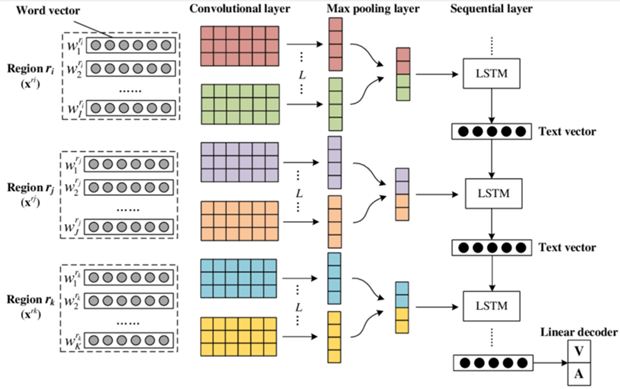
\includegraphics[width=0.9\linewidth]{CNN-LSTM.png}
    \caption{CNN-LSTM}
    \label{fig:circle}
\end{figure}

LSTM (long short-term memory, дословно (долгая краткосрочная память) — тип рекуррентной нейронной сети, способный обучаться долгосрочным зависимостям. 

LSTM были представлены в работе [Hochreiter & Schmidhuber (1997)]. Эта архитектура была создана для устранения проблемы долгострочных зависимостей. Пример: Я вырос во Франции … Я свободно говорю на французском.

\begin{figure}[!tbh]
    \centering
    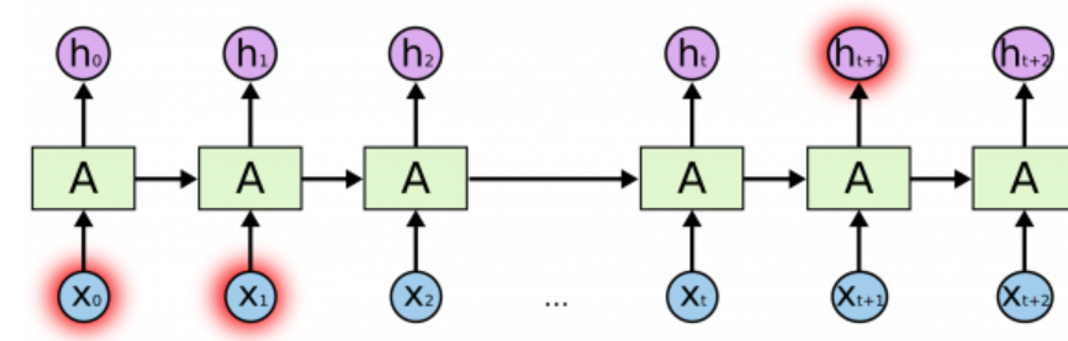
\includegraphics[width=0.9\linewidth]{2.png}
    \caption{LSTM}
    \label{fig:circle}
\end{figure}

Все рекуррентные нейронные сети имеют форму цепочки повторяющихся модулей нейронной сети. В простой сети там находится один модуль tanh, в рекурентной же находится 4 модуля.

\begin{figure}[!tbh]
    \centering
    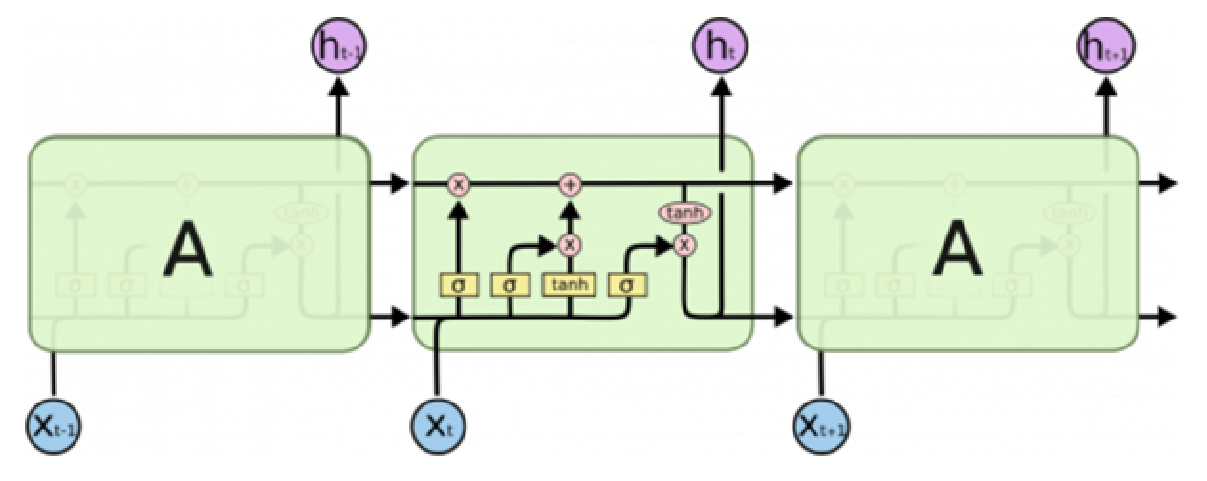
\includegraphics[width=0.9\linewidth]{3.png}
    \caption{LSTM}
    \label{fig:circle}
\end{figure}

Ключевым понятием LSTM является состояние ячейки: горизонтальная линия, проходящая через верхнюю часть диаграммы. В LSTM уменьшает или увеличивает количество информации в состоянии ячейки, в зависимости от потребностей. Для этого используются тщательно настраиваемые структуры, называемые гейтами. Гейт — это «ворота», пропускающие или не пропускающие информацию. Гейты состоят из сигмовидного слоя нейронной сети и операции поточечного умножения. Соотвественно каждая операция изменяет состояние ячейки в зависимости от нужд. Приведенный пример являет собой классическую lstm однако есть определенные модификации которые добавляю дополнительные операции в каждую ячейку.

\section{Набор данных}
В качестве данных для обучения используется набор данных RuREBus. Датасет представляет собой набор из 280 миллионов токенов, основанных на текстах Министерства экономического развития, инвестиций, туризма и внешних связей Российской Федерации и её субъектов. Часть датасета размечена вручную. Корпус представляет собой различные отчеты региональных органов о проделанной работе и запланированных мероприятиях, а также прогнозы и планы на будущее. Некоторое подмножество корпуса размечено специальными именованными сущностями (8 классов) и семантическими отношениями на них (11 классов).

Типы сущностей: 

1) MET (metric) – численный индикатор\показатель, объект, на котором определена операция сравнения. 
Примеры: Производительности труда, плановых и фактических значений показателей, сейсмичность территории, вероятность возникновения нарушения, экономического роста, степень износа здания.

2) ECO (economics) – экономическая сущность (из тех, что не подходят под определение MET) или объект инфраструктуры. 
Примеры: Биологических ресурсов, инновационного потенциала, внутреннего рынка, запасов и резервов продукции камчатских производителей, ресурсной базы рыболовства, частные компании
 
3) BIN (binary) – одноразовое действие бинарная характеристика (есть или нет) 
Пример: Создание, Строительство, Оказание, Обеспечение, Развитие, Приобретение, Формирование, Диверсификация, Вовлечение, Освоение, 

4) CMP (compare) - сравнительная характеристика. 
Примеры: Повышение, Насыщение, Увеличение, Повышению, Снизит, Получит развитие, Активизация, Превышает аналогичный показатель, Превышает их пропускную способность. 

5) QUA (qualitative) – качественная характеристика. 
Примеры: Стабильность, Ограниченность, Высокая, Неэффективная, Ограниченный, Большое, Склонен к самовозгоранию. 

6) ACT (activity) — принимаемые меры, проводимые мероприятия (часто сочетается с BIN: проводится [BIN] ремонт внутренних помещений [ACT], запущен [BIN] образовательный проект [ACT]). 
Примеры: Профилактика наркомании, Профилактика сиротства, Оповещение граждан о предстоящих мероприятиях по трудоустройству, Антинаркотические акции, Психолого-педагогическая помощь, Операции "МАК", «КАНАЛ" 

7) INST (institutions) — различные учреждения, заведения, структуры и организации 
Примеры: Учреждения культурно-досугового типа, центр Досуга и Творчества, этно-культурный центр, Сеть муниципальных учреждений культуры, Организации поддержки семьи и детства. 

8) SOC (social) – социальный объект. 
Примеры: Населения страны, специалистами и кадрами рабочих профессий, кадровая система, система льгот и преференций, профессиональных кадров.

Типы отношений: 

1) Текущее положение дел;

2) Реализованные изменения/итоги (о прошлом);

3) Прогнозы;

4) Цели;

5) Задачи.


\section{Эксперименты}
This section should include several subsections.
\subsection{Метрики}
Что касается оценки качества моделей, то тут используются стандартные метрики – точность, полнота и F-мера. 

Precision, recall и F-мера

Для оценки качества работы алгоритма на каждом из классов по отдельности введем метрики precision (точность) и recall (полнота).


$$\large precision = \frac{TP}{TP + FP}$$



$$\large recall = \frac{TP}{TP + FN}$$

Существует несколько различных способов объединить precision и recall в агрегированный критерий качества. F-мера (в общем случае $\ F_\beta$) — среднее гармоническое precision и recall :


$$\large \ F_\beta = (1 + \beta^2) \cdot \frac{precision \cdot recall}{(\beta^2 \cdot precision) + recall}$$


$\beta$ в данном случае определяет вес точности в метрике, и при $\beta = 1$ это среднее гармоническое (с множителем 2, чтобы в случае precision = 1 и recall = 1 иметь $\ F_1 = 1$)

F-мера достигает максимума при полноте и точности, равными единице, и близка к нулю, если один из аргументов близок к нулю.

Precision можно интерпретировать как долю объектов, названных классификатором положительными и при этом действительно являющимися положительными, а recall показывает, какую долю объектов положительного класса из всех объектов положительного класса нашел алгоритм.

Единицей для расчета этих метрик считается сущность, а не слово, то есть точность определяется как отношение количества правильно распознанных сущностей и количества распознанных сущностей, а полнота – как отношение правильно распознанных сущностей и количества сущностей в золотом стандарте. 

F-мера объединяет в себе две предыдущие метрики.
Из-за сегментации оценка качества модели осложняется, поскольку при обучении моделей мы используем слова, а для оценки – целые сущности. По этой причине если в нашем корпусе есть выражение Leamington Spa, а система определяет только Leamington – это уже ошибка.


\subsection{Experiment Setup}
Secondly, you need to describe the design of your experiment, e.g. how many runs there were, how the data split was done. The important details of your model, like hyper-parameters used in the experiments, and so on.


\section{Результаты}
В качестве результата была реализована сеть CNN-LSTM для решении задачи NER на датасете RuREBus. Были получены удовлетворительные результаты и доказано что модель способна обучаться.

Результаты работы нейросети представлены на графиках.

\begin{figure}[!tbh]
    \centering
    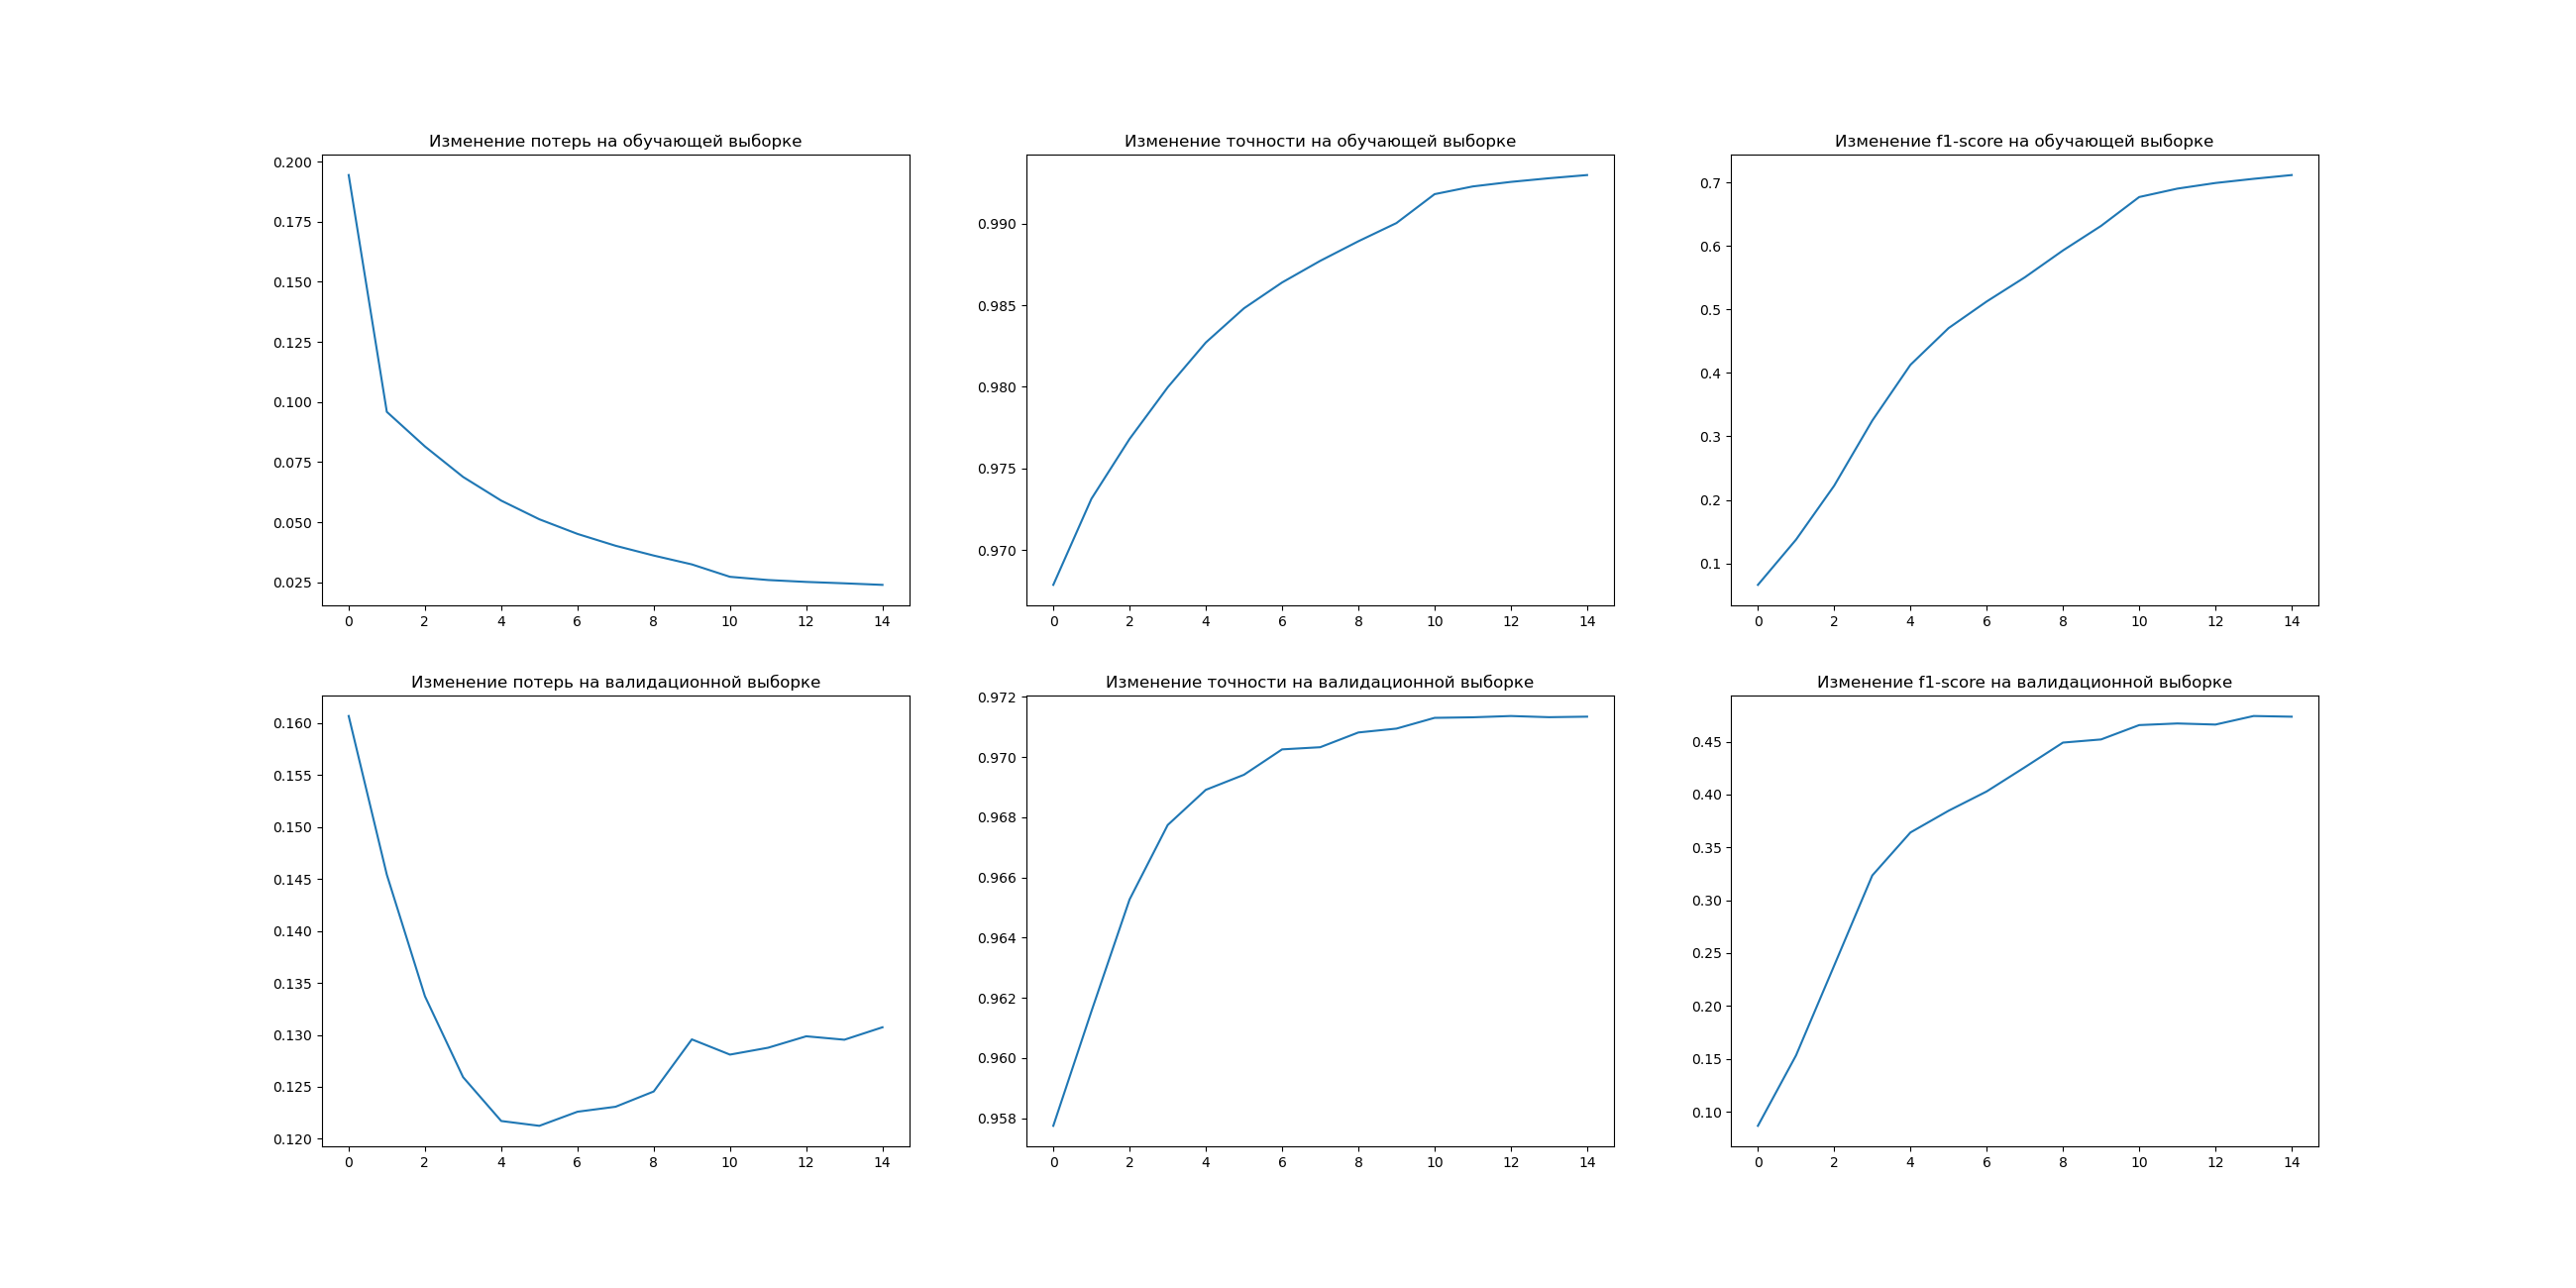
\includegraphics[width=0.9\linewidth]{res.png}
    \caption{результаты работы алгоритма}
    \label{fig:circle}
\end{figure}

Результат работы программы на тексте представлен ниже: 

\begin{table}[tbh!]
    \centering
    \begin{tabular}[t]{l|l}
         &  f-score\\
        Наше решение & 0.3386\\
        R-BERT & 0.464 \\
        BertForMultitaskLearning & 0.561 \\
    \end{tabular}
    \caption{Результаты нашего подхода и других участников соревнования}
    \label{tab:результаты нашего подхода и других участников соревнования}
\end{table}


\section{Заключение}
В результате реализации проекта была получена программная реализация алгоритма выявления сущностей из документов муниципальных структур при помощи глубокого обучения. Цель работы достигнута. 

В процессе были выполнены все поставленные в начале задачи.  Был подобран датасет, который включает в себя 280 млн токенов из документов министерства экономического развития, которые размечены вручную.

 Выбран наиболее подходящий метод решения поставленной задачи: CNN-LSTM.
Получена программная реализация алгоритма. Проведено тестирование и анализ результатов работы программы на реальных данных. Сформирован отчет о проделанной работе.
\bibliographystyle{apalike}
\bibliography{lit}
\end{document}

